\documentclass{beamer}
\usetheme{Frankfurt}

\usepackage{listings}

\newcommand{\todo}[1]{\alert{TODO #1}}

\title{Introduction}
\subtitle{Lecture 1 \\ Computer Security DD2395}
\author[R. Guanciale]{
  Roberto Guanciale\\
  robertog@kth.se
}
\date{2014-11-03}
\begin{document}

\begin{frame}[plain]
  \titlepage
\end{frame}

\begin{frame}{Outline for Today}
  \begin{itemize}
    \item About me
    \item About the course
    \item About you
    \item About computer security
  \end{itemize}
\end{frame}

\begin{frame}{About Roberto Guanciale}
  \begin{itemize}
    \item Assistant professor in Computer Security
    \item Research on formal verification
    \item Enthusiast software developer
    \item robertog@kth.se
      \begin{itemize}
      \item \alert{Always} use the e-mail subject: [DD2395] ...
      \end{itemize}
    \item use KTH social for questions
    \item Office: level 5, room 4525
    \item You are welcomed (no booking required, no fee)\\
      Wednesday 14:00-15:00
  \end{itemize}
\end{frame}

\begin{frame}{General Goals}
  \begin{itemize}
    \item Learn about security concepts
    \item Have tools and methods to reason about security
    \item Spot threats, vulnerabilities
    \item Know, propose and evaluate counter-measures
    \item Present concepts to others 
  \end{itemize}
\end{frame}

\begin{frame}{Learning Outcomes}
  You should be able to
  \begin{itemize}
    \item Explain the basic computer security terminology and concepts and use them correctly
    \item Analyse and design programs by a security point of view
    \item Analyse and design systems by a security point of view
    \item Describe existing counter-measures
    \item Compare counter-measures and evaluate their side-effects
    \item Find and apply documentation of security-related problems and tools
    \item Present and explain their reasoning to others
  \end{itemize}
\end{frame}



\begin{frame}{About the course}
  Lectures and Labs
  \begin{itemize}
    \item From now until December
    \item 3 Credits Lab + 3 Credits Examination
    \item Labs start November 11
    \item Starts lab in advance
    \item CINEK students have W and S labs in period 3
  \end{itemize}
\end{frame}


\begin{frame}{People}
  \begin{itemize}
    \item Course leader/exams: Roberto Guanciale
    \item Guest Lectures: 
      Martin Swende,
      Erik Hjelmvik,
      Hind Chfouka
    \item Lab assistants: 
      Benjamin Greschbach,
      Guillermo Rodriguez Cano,
      Hamed Nemati,
      Jan Elffers,
      Andreas Lindner
  \end{itemize}
\end{frame}

\begin{frame}{Course info and breaking news}
  \begin{itemize}
    \item Check course website regularly for updates!
    \item DD2395 on KTH Social
    \item https://www.kth.se/social/course/DD2395/
    \item \alert{Confirm your registration for the course}
      \begin{itemize}
        \item on ``my pages'' when logged into KTH
      \end{itemize}
    \item Check KTH Social Schedule for times and places
  \end{itemize}
\end{frame}


\begin{frame}{Main didactic material}
  \begin{itemize}
  \item William Stallings and Lawrie Brown, Computer Security:
    Principles and Practice, published by Pearson 
  \item Ross Anderson, Security Engineering, Free online
  \item KTH-social for links/papers/additional material
  \end{itemize}
\end{frame}

\begin{frame}{Language}
  \begin{itemize}
  \item Lectures/Mails/Website in English
  \item Exam English/Swedish
  \end{itemize}
\end{frame}

\begin{frame}{Lab Exercises}
  \begin{itemize}
    \item See KTH Social for times and rooms
    \item Instructions on web site
    \item 4 different exercises
      \begin{enumerate}
        \item on GnuPG, remote or at CSC
        \item on iptables/firewalls, at CSC
        \item on web attacks, remote or at CSC
        \item presentation at CSC, report, assess
      \end{enumerate}
  \end{itemize}
\end{frame}

\begin{frame}{Lab 3: Web attacks}
  \begin{itemize}
  \item Difficult: mastering several techniques
  \item self-assessment questions
    \begin{itemize}
      \item HTTP protocol basics: GET vs POST request?
      \item HTML basics: display a form with one input field and a
        submit button.
      \item Javascript basics: trigger a click event for a button with
        the id 'xxx' one second after the page is loaded
      \item SQL basics: combine the result from two different SELECT queries
    \end{itemize}
  \end{itemize}
\end{frame}

\begin{frame}{Lab 4: Seminar}
  \begin{itemize}
    \item Presentation and demo on computer security 
      topic in a seminar
    \item Groups of 2-3 students
    \item Topics will be published on the website
    \item You can suggest additional topics
    \item Group seminars, signup on course website
  \end{itemize}
\end{frame}

\begin{frame}{Groups}
 Only the G lab is done individually, all other labs
are done in groups of 2-3. You can form the
groups yourselves for each lab, find partners on
KTH Social or meet at the blackboard during the
lecture break to coordinate
\end{frame}

\begin{frame}{Deadlines}
  Fridays, at 5pm
  \begin{itemize}
    \item 13.11. F lab registration
    \item 20.11. G lab completion, S topic registration
    \item 27.11. S time registration, W lab registration
    \item 04.12. S report completion
    \item 11.12. F lab completion, S peer-review feedback completion
    \item 17.12. S, W lab completion (Except CINEK)
  \end{itemize}
\end{frame}


\begin{frame}{Exam}
  \begin{itemize}
  \item January 16, 2016
  \item \alert{Mandatory} registration 
  \item Re-exam in June 2016
  \item Oral exam for exchange students in December,
    sign up on KTH Social
  \end{itemize}
\end{frame}

\begin{frame}{Lectures Content}
  \begin{tabular}{cl|cl}
    01 & Admin, Intro [Ch.1] &         09 & Denial of Service [8] \\
    02 & OS/Networking  &              10 & Multi-level security [10] \\
    03 & Cryptography [2,20] &         11 & Buffer overflows [11] \\
    04 & Authentication [3] &          12 & Social engineering \\
    05 & Intrusion detection [8] &     13 & Network forensic (Guest) \\
    06 & Web security (Guest) &        14 & SW security \\
    07 & Firewalls [9]  &              15 & ? + Certification (Guest) \\
    08 & Malware [7] \\
    & & &\\
    & Secure multiparty computation & & Formal verification\\
    & Game theory & & Side channels
  \end{tabular}
\end{frame}




\begin{frame}{Assessment}
  \begin{itemize}
  \item 6 ECTS in total, $\sim$ 160 hours of work 
  \item 3 ECTS Labs $\in \{pass,fail\}$, no grades
  \item bonus points for exam (once) when bonus 
    requirements of lab fulfilled, see lab descriptions
  \item 3 ECTS Exam $\in [A \dots F]$
  \end{itemize}
\end{frame}

\begin{frame}{Grading criteria}
  \begin{itemize}
  \item Analyse and design systems by a security point of view
    \begin{itemize}
    \item E - know threats to confidentiality, integrity,
      and availability of well studied systems\\
      (e.g. TCP, IP, Message authentication codes, Operating systems)
    \item C - recognise threats to confidentiality, integrity, and
      availability of a new system\\ (e.g. formally demonstrate why a
      hash function is not secure)
    \item A - select counter-measures to identified threats and argue
      their effectiveness\\
      (e.g. correct a network protocol to prevent a security threat,
      design a system to include the selected countermeasures)
    \end{itemize}
  \end{itemize}
\end{frame}

\begin{frame}{Grading criteria}
  \begin{itemize}
  \item Analyse and design programs by a security point of view
    \begin{itemize}
    \item E - analyse small pieces of code or system descriptions in
      terms of their security
    \item C - identify vulnerabilities of such code or descriptions
      and predict their corresponding threats
    \item A - select counter-measures to identified threats and argue
      their effectiveness
    \end{itemize}
  \end{itemize}
\end{frame}

\begin{frame}{Grading criteria}
  \begin{itemize}
    \item Explain the basic computer security terminology and concepts and use them correctly
    \item Describe existing counter-measures
    \item Compare counter-measures and evaluate their side-effects
    \item Find and apply documentation of security-related problems and tools
    \item Present and explain their reasoning to others
    \begin{itemize}
    \item E - only
    \end{itemize}
  \end{itemize}
\end{frame}


\begin{frame}{Written exam}
  \begin{itemize}
\item Analize and design systems by a security point of view\\
E level: e.g. describe the principle of IP spoofing\\
C level: e.g. identify threat in a new network protocol\\
A level: e.g. extend a network protocol to support authentication
\item Analize and design programs by a security point of view\\
E level: e.g. identify a buffer overflow\\
C level: e.g. correct the program]]
A level: e.g. write an exploit that uses the bug to bypass a password check
\item Describe existing counter-measures\\
E level: e.g. describe the difference between a stateless and stateful firewall
\item Compare counter-measures and evaluate their side-effects\\
E level: e.g. compare two authentication protocols
\item Explain the basic computer security terminology and concepts and use them correctly\\
E level: e.g. Exampliofy high and low impact losses of confidentiality
  \end{itemize}
  \end{frame}


\begin{frame}{Final grade}
  \begin{itemize}
  \item E: 75\% of E-questions correct
  \item D: 75\% of E-questions correct, 50\% C-questions correct
  \item C: 75\% of E-questions correct, 75\% C-questions correct
  \item B: 75\% of E-questions correct, 75\% C-questions correct, 50\%
    A-questions
  \item A: 75\% of E-questions correct, 75\% C-questions correct, 75\%
    A-questions. Bonus point
  \end{itemize}
\end{frame}

\begin{frame}{Accounts}
  \begin{itemize}
  \item Needed for lab exercises
  \item Who doesn't have an account and access card?
  \item Go to the service center
  \end{itemize}
\end{frame}

\begin{frame}{Course Responsible Students }
  \begin{itemize}
  \item Select 2 students amongst yourselves 
  \item Introduce yourselves to me after the lecture 
  \end{itemize}
\end{frame}


\begin{frame}{Next Courses}
  \begin{itemize}
  \item Foundations of Cryptography with Douglas Wikstr\:om
  \item Software Security with Dilian Gurov
  \item Networking Security courses with Panos
    Papadimitratos at EES
  \end{itemize}
\end{frame}

\begin{frame}{Honor}
  \begin{itemize}
  \item CSC Honor code +
  \item \alert{Do not attack a running system 
    without the consent of the owner 
    and the users}
  \item Defense Against the Dark Arts
  \end{itemize}
  \center{
  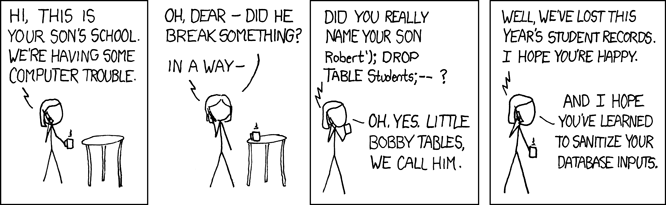
\includegraphics[width=0.7\linewidth]{exploits_of_a_mom}
  }
\end{frame}

\begin{frame}{Questions}
  \begin{itemize}
  \item ?????????????????????????
  \end{itemize}
\end{frame}


%%%%%%%%%%%%%%%%%%%%%%%%%%%%%%%%%%%%%%%%%%%%%%%%%%%%%%%%%%%%%%%%%%%%%%%%%%%

\begin{frame}{Overview}
  \begin{itemize}
  \item \alert{Computer Security}: protection afforded to an 
    automated information system in order to attain 
    the applicable objectives of preserving
    
    \begin{itemize}
    \item integrity (data/system)
    \item availability
    \item confidentiality (data/privacy)
    \end{itemize}
of  information system resources, including
 
\begin{itemize}
  \item hardware
  \item software
  \item firmware
  \item information/data
  \item telecommunications
\end{itemize}
  \end{itemize}
\end{frame}


\begin{frame}{Key Security Concepts}
  \begin{center}
    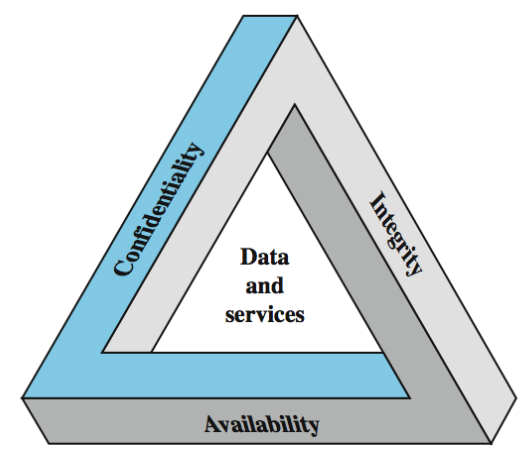
\includegraphics[width=0.7\linewidth]{concepts}
  \end{center}
\end{frame}

\begin{frame}{Security Myth}
  
  \begin{itemize}
\item   ``The only secure computer is one that's unplugged, locked in a safe,
  and buried 20 feet under the ground in a secret location...'' --
  Dennis Huges, FBI.
\item<2-> Only if you relax availability
  \end{itemize}
\end{frame}

\begin{frame}{Additional concepts}
  \begin{itemize}
  \item Authenticity
  \item Accountability
  \end{itemize}
\end{frame}  

\begin{frame}{Levels of impact}
  \begin{itemize}
  \item Low
    \begin{itemize}
      \item Confidentiality of student list
      \item Integrity of on-line pools
      \item Availability of a node in peer-to-peer file sharing
    \end{itemize}
  \item Moderate    
    \begin{itemize}
      \item Confidentiality of student grade
      \item Integrity of a web forum
    \end{itemize}
  \item High
    \begin{itemize}
      \item Availability of SCADA systems
      \item Integrity of financial transactions
    \end{itemize}
  \end{itemize}
\end{frame}

\begin{frame}{Challenges}
  \begin{itemize}
  \item Security can be hard to achieve. Why? 
  \item Think about it for 2 min. 
  \item Turn to your neighbor and discuss for 3 min.
  \end{itemize}
\end{frame}
 
\begin{frame}{Computer Security Challenges}
  \begin{itemize}
\item not simple in complex systems 
\item must consider potential attacks 
\item procedures used counter-intuitive 
\item involve several algorithms and secret info 
\item must decide where to deploy mechanisms 
\item battle of wits between attacker / admin 
\item not perceived as benefit until fails 
\item requires regular monitoring 
\item too often an after-thought 
\item regarded as impediment to using system
  \end{itemize}
\end{frame}


\begin{frame}{Security Terminology}
  \begin{center}
    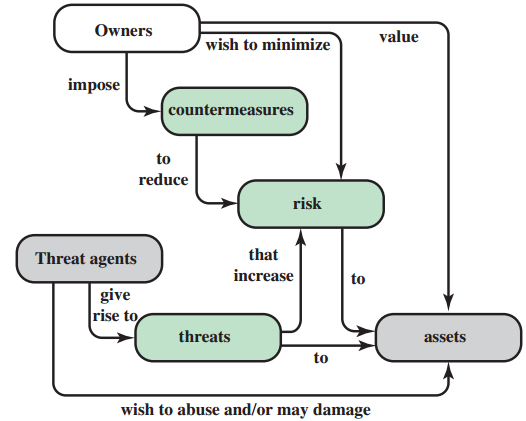
\includegraphics[width=0.7\linewidth]{terminology}
  \end{center}
\end{frame}

\begin{frame}{Security Terminology}
  \begin{center}
    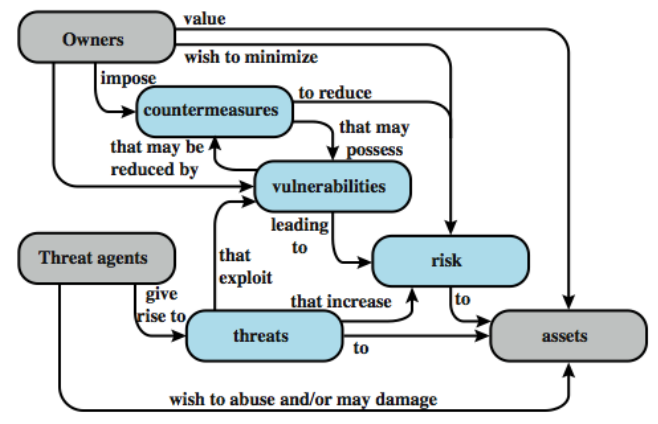
\includegraphics[width=0.7\linewidth]{terminology2}
  \end{center}
\end{frame}

\begin{frame}{Vulnerabilities and Attacks }
  \begin{itemize}
    \item vulnerabilities: system resources  may 
      
      \begin{itemize}
        \item be corrupted (loss of integrity) 
        \item become leaky (loss of confidentiality) 
        \item become unavailable (loss of availability) 
      \end{itemize}
    \item attacks are threats carried out and may be 
      \begin{itemize}
        \item passive
        \item active
        \item insider
        \item outsider
      \end{itemize}
  \end{itemize}
\end{frame}

\begin{frame}{Countermeasures}
  
  \begin{itemize}
    \item means used to deal with security attacks 
      
      \begin{itemize}
        \item prevent 
        \item detect 
        \item recover 
      \end{itemize}
    \item may result in new vulnerabilities 
    \item will have residual vulnerability 
    \item goal is to minimize risk given constraints
  \end{itemize}
\end{frame}


\begin{frame}{Threat Consequences}
  \begin{itemize}
    \item unauthorized disclosure (confidentiality) 
      \begin{itemize}
        \item exposure, interception, inference, intrusion 
        \end{itemize}
      \end{itemize}
  \begin{itemize}
    \item deception (integrity/authenticity/accountability)
      \begin{itemize}
        \item masquerade, falsification, repudiation 
        \end{itemize}
      \end{itemize}
  \begin{itemize}
    \item disruption (availability/integrity)
      \begin{itemize}
        \item incapacitation, corruption, obstruction 
        \end{itemize}
      \end{itemize}
  \begin{itemize}
    \item usurpation (system integrity)
      \begin{itemize}
      \item misappropriation, misuse
      \end{itemize}
    \end{itemize}
\end{frame}

\begin{frame}{Scope of Computer Security}
  \begin{center}
    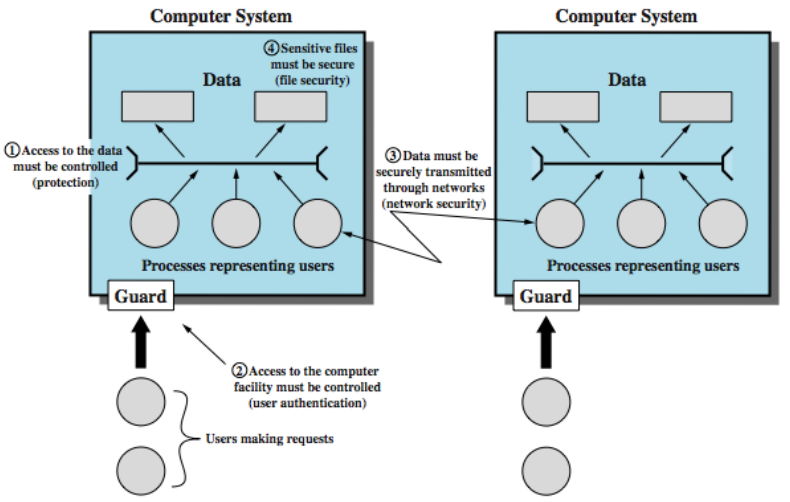
\includegraphics[width=0.8\linewidth]{securityScope}
  \end{center}
\end{frame}

\begin{frame}{Network Security Attacks}
  \begin{itemize}
    \item  classified as passive or active 
    \item  passive attacks are eavesdropping 
      \begin{itemize}
      \item release of message contents 
      \item traffic analysis 
      \item are hard to detect so aim to prevent 
    \end{itemize}
    \item active attacks modify/fake data 
      \begin{itemize}
      \item masquerade 
      \item replay 
      \item modification 
      \item denial of service 
      \item hard to prevent so aim to detect 
    \end{itemize}
    \end{itemize}
\end{frame}

\begin{frame}{Security Functional Requirements}
  \begin{itemize}
  \item technical measures: 
    \begin{itemize}
      \item access control; identification \& authentication; system \& 
      communication protection; system \& information integrity 
    \end{itemize}
  \item management controls and procedures 
    \begin{itemize}
      \item awareness \& training; audit \& accountability; certification, 
      accreditation, \& security assessments; contingency planning; 
      maintenance; physical \& environmental protection; planning; 
      personnel security; risk assessment; systems \& services 
      acquisition 
    \end{itemize}
  \item overlapping technical and management: 
    \begin{itemize}
      \item configuration management; incident response; media protection
    \end{itemize}
  \end{itemize}
\end{frame}

\begin{frame}{X.800 Security Architecture}
  \begin{itemize}
    \item X.800, Security Architecture for OSI 
    \item systematic way of defining requirements for 
    security and characterizing approaches to 
    satisfying them 
    \item defines: 
      \begin{itemize}
        \item security attacks - compromise security 
        \item security mechanism - act to detect, prevent, 
        recover from attack 
        \item security service - counter security attacks 
      \end{itemize}
  \end{itemize}
\end{frame}

\end{document}




%%% Local Variables: 
%%% mode: latex
%%% TeX-master: t
%%% End: 
